\begin{lstlisting}[float=hpb,label=lst:sdg-intro,
  caption={Configurable program using load-time variability which results in the SDG in \autoref{fig:sdg-intro}}]
class Main {
  static Properties p = Properties.load("conf.prop");
  static boolean c0 = p.getProperty("c0", "").equals("on");
  static boolean c1 = p.getProperty("c1", "").equals("on");
  
  public static void main(String[] args) {
    A obj = new A();
    D d = new D();
    if(c0) {
      obj = new B();
      return;
    } else if(c1) {
      obj = new C();
    }
    int res = obj.foo(d);
    System.out.println(res);
  }
  
  class A {
    int foo(D d) {
      return 2;
    }
  }
  class B extends A {
    int foo(D d) {
      return d.bar() * d.bar();
    }
  }
  class C extends A {
    int foo(D d) {
      return 2 * d.bar();
    }
  }
  class D {
    int bar() {
      if(!c1)
        return 1;
      return 0;
    }
  }
}
\end{lstlisting}

\begin{figure}[hpb]
  \centering
    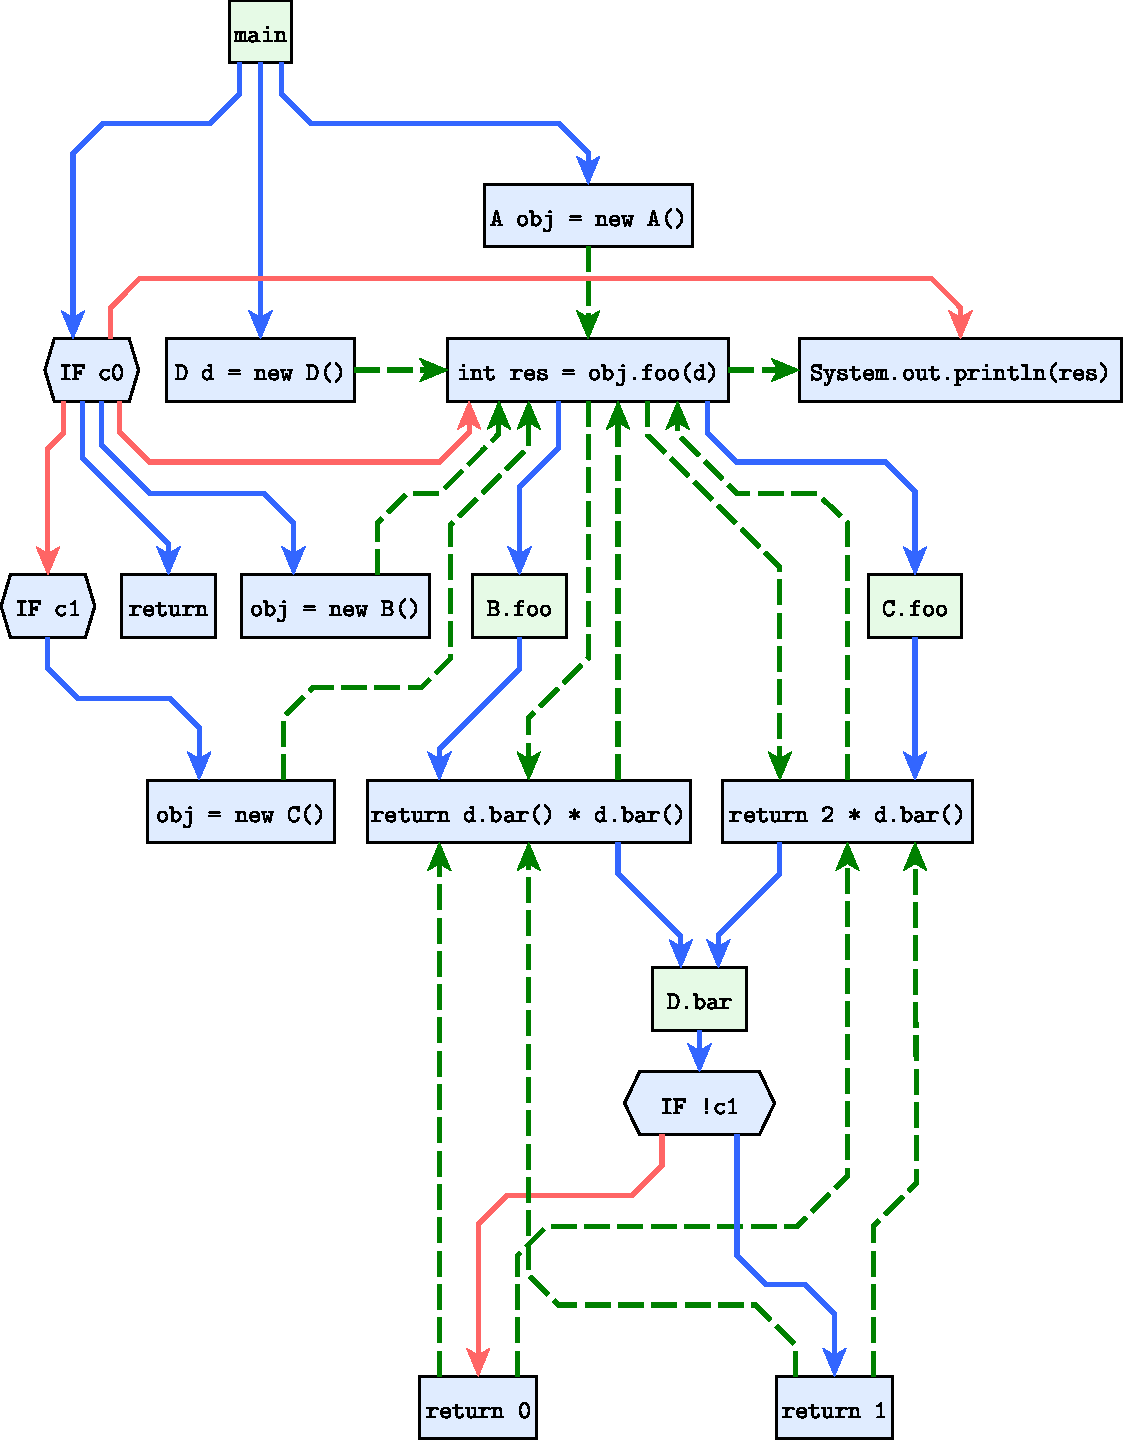
\includegraphics[scale=0.6]{sdgs/intro}
  \caption{SDG for the sample program in \autoref{lst:sdg-intro}}
  \label{fig:sdg-intro}
\end{figure}
